\section{Casos de prueba}
\label{sec:intro}

Para evaluar el comportamiento y fijar los parametros del algoritmo utilizamos los casos de prueba obtenidos de
\url{http://lipas.uwasa.fi/~timan/sudoku/}, los cuales estan ordenados en cuantro categorías: \textit{fácil, medio, difícil y ultra difícil}.

Nuestra heuristica logro encontrar el resultado en todos los casos de prueba en 
un tiempo inferior a los 5 minutos. En las categorias  \textit{fácil y medio} no 
se llegaba a la primer iteracion del mismo.

Esto significaba que el algoritmo estaba encontrando la solucion sin compartir 
la informacion entra las hormigas. 

Por lo tanto para fijar los parametros decidimos utilizar el caso de mayor dificultad. 

En un primer momento queriamos evaluar cuantas hormigas debiamos utilizar. 
Para esto dejamos fijo el número de ciclos ($20$) y fuimos variando la cantidad de hormigas. 
Este primer resultado nos llamo la atención, ya que al incremetar el numero de hormigas, no se modificaba el tiempo 
promedio utilizado para encontrar la respuesta asi como tampoco la cantidad de 
ciclos generales usados para encontrar la solucion. 

\begin{figure}[h]
	\centering
	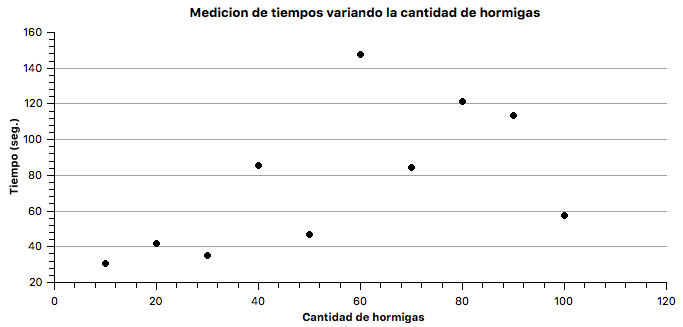
\includegraphics[scale=0.55]{./graficos/variacion_hormigas.png}
	\caption{Variación de cantidad de hormigas}
	\label{img:time_ants}
\end{figure}


Una segunda prueba fue variar el factor de evaporación, pensando que a mayor nivel de evaporación, 
menor la incidencia de las hormigas en el algoritmo y por lo tanto mayor seria el tiempo, o inclusive que no 
encontraria la solución.
Dejando fijo los ciclos ($20$) y la cantidad de hormigas ($10$) fuimos variando el factor de 
evaporacion, calculando el porcentaje de soluciones encontradas sobre un numero de corridas.  

\begin{figure}[h]
	\centering
	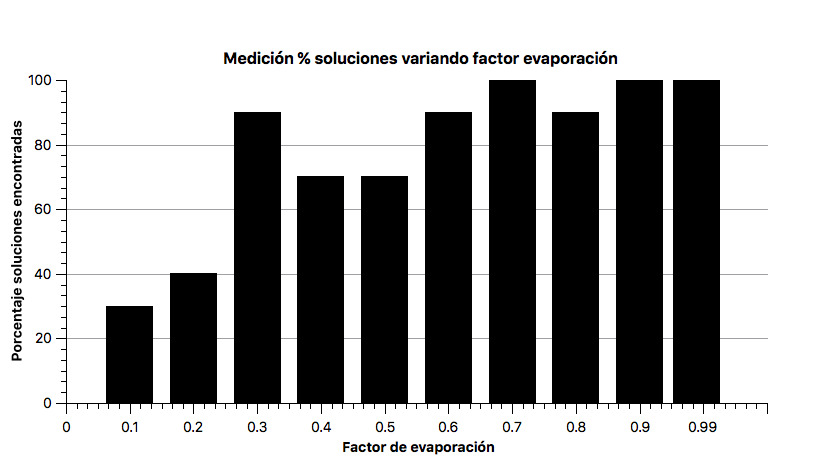
\includegraphics[scale=0.4]{./graficos/variacion_evaporacion.png}
	\caption{Variación del factor de evaporación}
\end{figure}

\newpage

Como podemos ver, con valores chicos del factor de evaporación, algunas instancias no 
encuentran la solucion optima al problema. Esto se debe a que se esta 
modificando demasiado la probabilidad de los digitos a ser elegidos en el trabajo de la hormiga, perjudicando al 
algoritmo. 

Debido a que a niveles alto de feromona el resultado del algoritmo no se veia perjudicado, 
la prueba que hicimos fue eliminar directamente el uso de 
la feronoma del algoritmo, y por lo tanto las hormigas no compartirian 
informacion. 

\begin{center}
  \begin{tabular}{ | l | c | c | c | c | c | c | c | c| c | c |}
    \hline
    Nro instancia &  1 & 2 & 3 & 4 & 5 & 6 & 7 & 8 & 9 & 10 \\  \hline
    Cant. digitos & 81 & 81 & 81 & 81 & 81 & 81 & 81 & 81 & 81 & 81 \\ \hline
    Tiempo (ms) & 83177 & 21203 & 19253 & 1769 & 32119 & 27440 & 39931 & 26452 & 11019 & 5297 \\
    \hline
  \end{tabular}
\end{center}

Sorprendentemente, el algoritmo no se vio afectado por estos cambios. Siempre 
encontro la solucion y en tiempos muy bajos.

Esto nos sorprendio bastante. Una primera hipotesis es que el caso de prueba utilizado no se lo 
suficientemente dificil para el algoritmo, ya que estabamos encontrando la 
solucion sin utilizar la feromona, y por otro lado otra posibilidad es que no se 
este utilizando la informacion de la feromona correctamente.

Decidimos entonces buscar instancias mas dificiles, y ncontramos un dataset \footnote{Problemas de la lista de 'top95' disponible en http://magictour.free.fr/top95} 
para hacer nuevas pruebas sobre nuestro algoritmo.

Por un lado corrimos el algoritmo utlizando la feormona, y por otra parte corrimos la version que no hace utilización  de 
la misma. Sobre un total de $10$ corridas verificamos en ambos casos que 
porcentaje de soluciones optimas fueron encontrados

\begin{center}
  \begin{tabular}{ | l | c | c |}
    \hline
     & Utilizando feromona & Sin utilizar \\  \hline
     \% Sol. encontradas & 20\% & 20\% \\ \hline
    Tiempo (ms) & 83177 & 21203 \\
    \hline
  \end{tabular}
\end{center}

Si bien podemos ver que esta instancia es mas dificil para nuestro algoritmo, 
también se desprende que la fermonona o bien no esta actuando correctamente o 
bien no esta ayudando por alguna razon al algoritmo. Sin embargo en ambos casos 
la solución fue encontrada al menos en una oportunidad. 


\newpage























